\documentclass{article}

\usepackage{amsmath, amssymb, amsfonts, amsthm, booktabs, verbatim, mathtools, listings, xcolor}
\usepackage{hyperref}
\usepackage{tikz}
\usetikzlibrary{arrows, shapes}

%\numberwithin{equation}{section}
\newtheorem{theorem}{Theorem}
\newtheorem{lemma}{Lemma}
\newtheorem{proposition}{Proposition}
\newtheorem{definition}{Definition}
\newtheorem{problem}{Problem}
\newtheorem{example}{Example}
\newtheorem{remark}{Remark}

% Surrounding angular brackets
\newcommand{\surang}[1]{\langle #1 \rangle}
\makeatletter
\newcommand{\@giventhatstar}[2]{#1\,\middle|\,#2}
\newcommand{\@giventhatnostar}[3][]{#1(#2\,#1|\,#3#1)}
\newcommand{\giventhat}{\@ifstar\@giventhatstar\@giventhatnostar}
\makeatother
\newcommand{\probof}[1]{\text{Pr}\left( #1 \right)}
\newcommand{\pdens}[1]{p\left( #1 \right)}
\newcommand{\variance}[1]{\text{Var}\left( #1 \right)}

\lstset{ %
  language=R,                     % the language of the code
  basicstyle=\footnotesize,       % the size of the fonts that are used for the code
  numbers=left,                   % where to put the line-numbers
  numberstyle=\tiny\color{gray},  % the style that is used for the line-numbers
  stepnumber=1,                   % the step between two line-numbers. If it's 1, each line
                                  % will be numbered
  numbersep=5pt,                  % how far the line-numbers are from the code
  backgroundcolor=\color{white},  % choose the background color. You must add \usepackage{color}
  showspaces=false,               % show spaces adding particular underscores
  showstringspaces=false,         % underline spaces within strings
  showtabs=false,                 % show tabs within strings adding particular underscores
  frame=single,                   % adds a frame around the code
  rulecolor=\color{black},        % if not set, the frame-color may be changed on line-breaks within not-black text (e.g. commens (green here))
  tabsize=2,                      % sets default tabsize to 2 spaces
  captionpos=b,                   % sets the caption-position to bottom
  breaklines=true,                % sets automatic line breaking
  breakatwhitespace=false,        % sets if automatic breaks should only happen at whitespace
  title=\lstname,                 % show the filename of files included with \lstinputlisting;
                                  % also try caption instead of title
  keywordstyle=\color{blue},      % keyword style
  commentstyle=\color{red},   % comment style
  stringstyle=\color{black},      % string literal style
  escapeinside={\%*}{*)},         % if you want to add a comment within your code
  morekeywords={*,...}            % if you want to add more keywords to the set
} 

\begin{document}
\tikzstyle{int}=[draw, fill=blue!20, minimum size=2em]
\tikzstyle{init} = [pin edge={to-,thin,black}]

\tableofcontents

\section{Hierarchical Modeling}

Hierarchical modeling was covered much earlier in this class, but it shows up
prominently through the second half of this course as well and so a refresher
is rather in order.
Moreover, it shows up all the time in the real world and industry.

Hierarchical modeling is a way of expanding the expressiveness of your model while keeping it computationally feasible.
For a hierarchical model of $n$ levels, for each $i$th level, we assume that that level has priors whose parameters are drawn from the $i + 1$-th level (the priors for the $n$th level are fixed at model creation time and termed the ``hyperpriors'')
In most applications we stick with $n = 2$ (and certainly do so in this class).
See Remark~\ref{remark:hierarchical_models} for more.

\begin{remark}
	\label{remark:hierarchical_models}
	While hierarhical models can be developed in much greater generality,
	in class and in practice they look something like the following $2$ levels.

	For purposes of notation, we'll often use $\phi$ to denote parameters
	of the top, second level (also often called the ``hyperparameters'')
	and use $\theta$ to denote the parameters of the lower level.

	Often we think of $\theta$ as being multiple $\theta _i$s each
	independently drawn from the distribution parametrized by $\phi$.  In
	turn for each $\theta _i$ multiple $y _{i, j}$ are drawn from the
	distribution parametrized by $\theta _i$.

	See Figure~\ref{fig:hierarchical_model} for a graphical illustration of this.
\end{remark}
\begin{figure}
	\centering
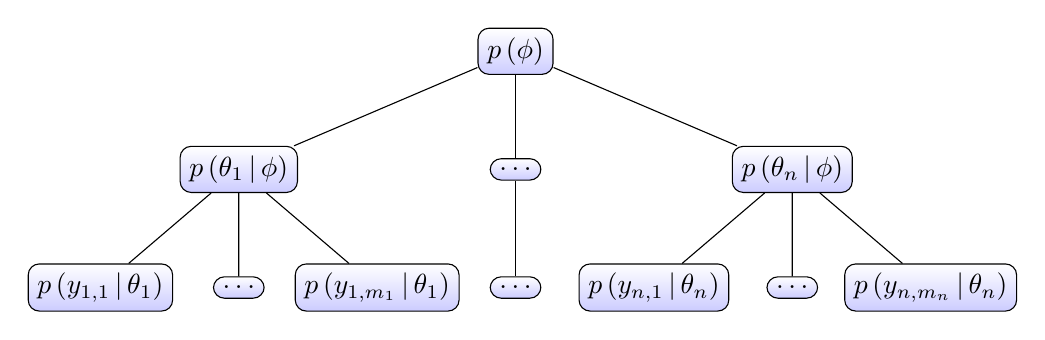
\begin{tikzpicture}[level/.style={sibling distance=10em/#1},
  every node/.style = {shape=rectangle, rounded corners,
    draw, align=center,
    top color=white, bottom color=blue!20}]]
  \node {$\pdens{\phi}$}
    child { node {$\pdens{\giventhat*{\theta _1}{\phi}}$} 
        child { node {$\pdens{\giventhat*{y_{1, 1}}{\theta_1}}$} }
        child { node {$\ldots$} }
	child { node {$\pdens{\giventhat*{y_{1, m_1}}{\theta_1}}$}}
    }
    child { node {$\ldots$} 
        child { node {$\ldots$} }
    }
    child { node {$\pdens{\giventhat*{\theta _n}{\phi}}$} 
        child { node {$\pdens{\giventhat*{y_{n, 1}}{\theta_n}}$} }
        child { node {$\ldots$} }
	child { node {$\pdens{\giventhat*{y_{n, m_n}}{\theta_n}}$}}
    };
\end{tikzpicture}
	\caption{A graphical illustration of a two-level hierarchical model. $\phi$ is the hyperparameter, the $\theta _i$s our parameters, and the $y _{i, j}$ are our observed data.}
	\label{fig:hierarchical_model}
\end{figure}

Hierarchical modeling gives us one crucial avenue of simplification, which is that \emph{each successive layer depends only its most immediate previous layer}.
For example, notice that the bottom layer of Figure~\ref{fig:hierarchical_model} has $\pdens{\giventhat*{y_{1, 1}}{\theta _1}}$, which is one specific example of Equation~\ref{eq:hierarchical_model}.
\begin{equation}
	\pdens{\giventhat*{y}{\theta, \phi}} = \pdens{\giventhat*{y}{\theta}}
	\label{eq:hierarchical_model}
\end{equation}
Equation~\ref{eq:hierarchical_model} is exactly what allows us to make hierarchical models tractable.

Note that for hierarchical models, generally we know
\begin{enumerate}
	\label{enum:hierarchical_model}
	\item 
		Our prior on $\phi$
	\item
		The distribution of $\theta$ conditioned on $\phi$
	\item
		The distribution of $y$ conditioned on $\theta$
\end{enumerate}
and the ``holy grail'' we are usually solving
for is a posterior marginal distribution of the hyperparameters, that is
$\pdens{\giventhat*{\phi}{y}}$.
Because everything ``flows down'' from the top level, having the posterior
marginal distribution of the hyperparameters lets us solve the lower levels of the
model by conditioning on the values of the upper levels.

General steps:
\begin{enumerate}
	\item 
		Begin by computing the (unnormalized) joint posterior (notice how we use Equation~\ref{eq:hierarchical_model} here):
		\begin{align*}
			\pdens{\giventhat*{\theta, \phi}{y}}
			&\propto \pdens{\theta, \phi} \pdens{\giventhat*{y}{\theta, \phi}}\\
			&= \pdens{\theta, \phi} \pdens{\giventhat*{y}{\theta}}\\
			&= \pdens{\phi} \pdens{\giventhat*{\theta}{\phi}} \pdens{\giventhat*{y}{\theta}}
		\end{align*}

		This form contains all the factors we generally have access to (see the steps outlined on page~\pageref{enum:hierarchical_model}) from the outset.
	\item
		Find $\pdens{\giventhat*{\theta}{\phi, y}}$, i.e. the conditional posterior density of our parameters.
		At this point, because $\phi$ is fixed, we are in the space of usual Bayesian inference (it may help to conjure up a new random variable $\theta' = \left( \giventhat*{\theta}{\phi} \right)$ whose prior is $\pdens{\giventhat*{\theta}{\phi}}$ and on which we're doing inference given $y$) and the same caveats apply.
		Do your best to set up your hierarchy so that $\pdens{\giventhat*{\theta}{\phi}}$ is a prior that is easy to update on given the likelihood function $\pdens{\giventhat*{y}{\theta}}$ (e.g. use a conjugate prior).
	\item
		Using $\pdens{\giventhat*{\theta}{\phi, y}}$ from the previous step, calculate the marginal posterior of our hyperparameters $\pdens{\giventhat*{\phi}{y}}$, i.e. the ``holy grail'' we were after in the first place.
		Often you can use the conjunction trick (see Appendix~\ref{section:computation_tricks} on page~\pageref{section:computation_tricks}) to get Equation~\ref{eq:hierarchical_marginal_easy} which you can use to compute the marginal.
		\begin{equation}
			\pdens{\giventhat*{\phi}{y}} = \frac{\pdens{\theta, \phi}{y}}{\pdens{\giventhat*{\theta}{\phi, y}}}
			\label{eq:hierarchical_marginal_easy}
		\end{equation}
		If that fails you'll need to turn to brute force integration.
\end{enumerate}

The standard example here is the normal-normal model.

We'll see more examples later on (e.g. Example~\ref{example:faculty} on
page~\pageref{example:faculty}) that integrate more knowledge of other things
as well.

\section{Model Comparison}

\section{Experimental Design and Missing Data}

\subsection{Propensity Scores}

\begin{definition}
	Given an inclusion vector $I = (I_0, I_1, \ldots, I_n)$, the $i$th propensity score is defined to be
	\begin{equation}
		\pi_i = \pdens{\giventhat*{I_i}{x}}
		\label{eq:propensity_def}
	\end{equation}
	that is the $i$th propensity score $\pi _i$ is the marginal distribution of the $ith$ component of the inclusion vector.
\end{definition}

What does it mean for the propensity scores to be a good summary of the data/inclusion vector?
It means
\begin{equation}
	\pdens{\giventhat*{I}{x}} = \pdens{\giventhat*{I}{\pi _1, \ldots, \pi _n}}
	\label{eq:propensity_is_good_1}
\end{equation}
or equivalently (assuming the existence of a PDF)
\begin{equation}
	\exists g: g(\pdens{\giventhat*{I_1}{x}}, \ldots, \pdens{\giventhat*{I_n}{x}}) = f(I_1, \ldots, I_n)
\end{equation}
where $f$ is the joint PDF of the inclusion vector components.
In other words, the propensity scores (marginal distributions) are a good
summary of the inclusion vector if the joint distribution over all components
can be completely determined by the marginal distributions of each component.

\begin{example}[Where propensity score is a good summary of the data]
	The easiest example of where the propensity score is a good summary of
	the data is when the components of the inclusion vector are independent
	from each other (because in that case the joint distribution is just
	the product of the marginals).

	An example of that is the simple random
\end{example}

\begin{example}[Missing fish]
\end{example}

\begin{example}[Exercise~8.5]
\end{example}

\section{Decision Analysis}

Decision analysis follows the following four steps (page~$238$ in Gelman et. al).
\begin{enumerate}
	\item 
		Enumerate the space of all possible decisions and outcomes $x$
	\item
		Determine the probability of $x$ for each decision $d$
\end{enumerate}

We have the Oscar problem from homework (and also the back of Chapter 9).

\begin{example}[Pizza Shop: \href{http://www2.gsu.edu/~dscgpz/mgs3100/exercise3.pdf}{http://www2.gsu.edu/~dscgpz/mgs3100/exercise3.pdf}]
You own a pizza shop in a downtown mini-mall. It is Saturday morning, and you
are trying to decide how many pizzas to make to meet today's lunch
hour demand. Based upon your experience with Saturdays, you think
that the probability of being able to sell 20 pizzas is 0.2, of
being able to sell 40 pizzas is 0.3, and of being able to sell 50 pizzas is
0.5.

Suppose a pizza sells for \$10 and has an incremental cost of
\$4.25. If you have leftover pizzas, you can sell them to the
homeless shelter for \$1.25 each. If demand exceeds the number of
pizzas you have prepared, every disappointed customer costs you \$0.25 worth of
lost customer goodwill. 

How many pizzas should you make?
\end{example}
\begin{proof}
	The payoff $P_n$ for $n$ pizzas with $M$ customers is calculated as
	\begin{equation}
		P_n = -4.25 n + 10 \min(M, n) + 1.25 \max(n - M, 0) - 0.25 \max(M - n, 0)
	\end{equation}
	The expected number of customers is $20 \cdot 0.2 + 40 \cdot 0.3 + 50 \cdot 0.5 = 41$.

	Therefore, the expected value of your payoff given $n$ pizzas made is
	\begin{align*}
		E(P_n) 
		&= E(-4.25 n + 10 \min(M, n) + 1.25 \max(n - M, 0) - 0.25 \max(M - n, 0))\\
		&= -4.25n + 10 \min(E(M), n) + 1.25 \max(n - E(M), 0) - 0.25 \max (E(M) - n, 0)\\
		&= -4.25n + 10 \min(41, n) + 1.25 \max (n - 41, 0) - 0.25 \max (41 - n, 0)
	\end{align*}

	If we squint at the maxes and mins, it's apparent that this is a monotonically increasing linear function up to $41$ and then sharply decreases afterwards.

	Therefore to maximize our expected payoff, we should make $41$ pizzas, which will give us a payoff of $235.75$.
	This should probably accord well with your intuition, make as many pizzas as expected people who will show up.

	In general if you have a linear combination of costs, you should always shoot to make as many pizzas as customers you think will show up (because expected value obeys linearity).
\end{proof}

\begin{example}
\end{example}

\section{Sampling Distributions}

Often Bayesian statistics results in distributions which are not analytically convenient to deal with (indeed outside of relying on conjugate priors this is the norm).
We therefore often turn to simulation via sampling to arrive at numerical solutions to our problems.

\begin{remark}
	Numerical approximation of Bayesian methods doesn't require sampling.

	The other way of doing things is numerical integration (given how little of
	this was covered in class, I would be surprised if it came up) to calculate
	both the normalizing constant (denominator in Bayes' Theorem) as well as
	various events of your posterior distribution.

	Sampling is often more convenient and flexible though than numerical approximation and is the current state of the art in statistical numerical methods.
\end{remark}

Sampling from a distribution, however, is not as trivial an exercise as it may seem at first.
Knowing the PDF of your distribution is necessary, but it may not be obvious how to go from a PDF to an actual sampling strategy.

Here we'll outline various strategies in roughly ``ascending'' order.
That is we'll start with fairly naive strategies, outline examples where they work well and then examples where they do not.
Then we'll present another strategy which deals with some of the shortcomings of the previous one.

That is not to say the final strategy we present is the absolute best strategy 

The method for sampling from a distributions generally all follow this layout:
\begin{enumerate}
	\item
		(Source Distribution):
		Have some sort of distribution (source distribution) from which you know how to sample and of which you know its (unnormalized) probability density function.
		We often implicitly assume alongside an explicitly listed source distribution the existence of a way to sample from the $\text{Uniform}(0, 1)$ distribution.
	\item
		(Target Distribution):
		Know the (unnormalized) probability density function of the distribution you wish to simulate (target distribution)
	\item
		(Translation Strategy):
		Figure out some way of translating draws of your source distribution to your target distribution based on the relationship between the former and latter's probability density function
\end{enumerate}

The only difference among our different simulation methods is the third point.

Note that these steps are not necessarily performed in this chronological order.
In particular, it is often the case that details of your target distribution and/or translation strategy influence which kind of source distribution you'd like to use.

\subsection{Grid Approximation}

The first method we'll briefly cover is grid approximation, which should be familiar from the very beginning of this course.
Here the source distribution is a discrete approximation with bounded support of your target distribution.
To actually sample from this source distribution, we then construct an inverse CDF of this discrete approximation.
We can then sample from a $\text{Uniform}(0, 1)$ distribution and then take the resulting samples and pass them to the inverse CDF to generate samples of our discrete approximation.

Here our translation strategy is more or less ``wave your hands'' and assume that your discrete approximation is a good approximation of your target distribution and therefore the sample generated from the discrete approximation is a good approximation of a sample generated from your target distribution.

\begin{itemize}
	\item[Pros:]
		\begin{enumerate}
			\item 
				Simple and straightforward, both to implement and in its theoretical justification.
			\item
				Any discrete approximation with bounded support can be made arbitrary close to the target distribution by simply decreasing the size of the discretization step and increasing the bounds of its support.
		\end{enumerate}
	\item[Cons:]
		\begin{enumerate}
			\item 
				Can be (potentially very) inaccurate in the presence of ``spiky'' target distributions and/or distributions that are ``spread out'' (i.e. that have significantly non-zero values over a large subset of its domain).
				This is a result of deficiencies in the discretization step and bounds of the support respectively.
			\item
				The solution to these deficiencies, i.e. decreasing the size of the discretization step and increasing the bounds of the support can drastically increase computational resources required to calculate the discrete inverse CDF, especially in the presence of multivariate distributions with many variates.
		\end{enumerate}
\end{itemize}

\subsection{Rejection Sampling}

The grid approximation method can be problematic because of its discrete and bounded nature, so why not try to tackle that by having a continuous source distribution?
That is exactly what the rejection sampling method does.

Our source distribution can be any distribution with the same domain as our target distribution so long as the source distribution can be scaled to always be larger than the target distribution.
That is if our source distribution has density function $g$ and our target distribution has density function $f$, there is a $k$ such that for all $x$ in our domain, $kg(x) \ge f(x)$.

\subsection{Markov Chain Monte Carlo}

The jump distributions we have almost always used in class and on our homework has been a state-independent jump distribution.
That is the jump distribution $J$ such that $J\left( \giventhat*{\theta ^\star}{\theta ^{s - 1}} \right) = J\left( \giventhat*{\theta ^\star} \right)$.

In the case of MCMC algorithms,

Note that such a jump distribution requires the full ratio function of the Metropolis-Hastings algorithm (and not the simplified symmetric version in just Metropolis)!
In particular
\begin{align*}
	J\left( \giventhat*{\theta ^\star}{\theta ^{s - 1}} \right)
	&= J\left( \theta ^\star \right)\\
	&\not= J\left( \theta ^{s - 1} \right)
\end{align*}
which means that our jumps are not symmetric.

\subsubsection{Gibbs Sampler}

The Gibbs sampler is great when we can break down

We can use the Gibbs sampler to help sample from
\begin{example}[Coagulation 11.6]
	\label{example:coagulation}
	We have a hierarchical normal model with a series of random variables $\theta$s $\theta_1, \ldots, \theta_n$ that all share a common variance $\sigma ^2$ from which we draw $y_{i, 1}, \ldots, y_{j, m} \sim _\text{iid} N(\theta _i, \sigma ^2)$.
	For each $\theta _i$, we have a prior such that $\theta _i \sim N(\mu, \tau ^2)$.
	Finally for $\mu$ we have a hyperprior of $\pdens{mu, \log \sigma ^2, \log \tau} \propto \tau$.

	Note that it is equivalent to say $\pdens{mu, \log \sigma ^2, \log \tau} \propto \tau$ and the joint distribution $mu, \log \sigma ^2, \tau$ is uniform.
\end{example}

\begin{example}[Faculty publication rates, Homework~4.5]
	\label{example:faculty}
	Imagine that we have a faculty of $n$ members at some university for which we have a simple random sample of $k$ faculty members and the number of publications they have made where $k < n$.
	Come up with a $95\%$ posterior interval for the total number of refereed publications 
	For one of our homework problems we had an extremely naive model for trying to infer 
\end{example}
\begin{proof}
\end{proof}

It is perhaps instructive to compare Example~\ref{example:coagulation} with the original problem in Section~5.4 of Gelman et al.
Note in that example we have $\sigma ^2$ fixed (instead of unknown) and have as a hyperprior instead $\pdens{mu, \tau} \propto \pdens{\tau}$ with a uniform marginal prior on $\tau$.

\begin{example}[Problem 11.1 on page~$291$ of Gelman et al.]
\end{example}

\begin{example}[Problem 11.4 on page~$292$ of Gelman et al.]
\end{example}

\begin{example}[Problem 11.6 on page~$292$ of Gelman et al.]
\end{example}

\appendix

\section{Computational Tricks}
\label{section:computation_tricks}

Analytically, Bayesian statistics is very simple.
There's only so many algebraic manipulations you can do.

Here is a short toolbox of what you might think of as ``rewrite rules'' that can often rewrite your equation to make it more tractable.
Comes in handy on tests, homework, and the real world alike.

\begin{enumerate}
	\item 
		Bayes' Rule: This one is pretty self-explanatory. Often comes in handy in its unnormalized version.
		\begin{equation}
			\pdens{\giventhat*{\theta}{y}} = \frac{\pdens{\theta} \pdens{\giventhat*{y}{\theta}}}{y} \propto \pdens{\theta} \pdens{\giventhat*{y}{\theta}}
		\end{equation}
	\item
	\item
		Condition Pruning: The hallmark of the hierarchical model, but often crops in decision analysis underlies the theory behind MCMC. 
		Stay on the lookout for when one event entails another or when one random variable depends on another only indirectly through an intermediate random variable.
	\item
		Recognition of integrals of 
\end{enumerate}<++>

\section{Rough order as covered in class}

\begin{enumerate}
	\item
	\item
	\item
\end{enumerate}

\end{document}
